\section{実験}





改造したMiniSatと実装した遺伝アルゴリズムを用いて実際に証明の作成を行なった。
主な実験として
\begin{enumerate}
    \item 遺伝アルゴリズムのパラメータを調整して、短い証明を作りやすくするための実験
    \item 調整を行なった遺伝アルゴリズムがどれぐらいの効果あるかをみる実験
    \item 最先端のソルバーと比べてどれぐらい短い証明が作れているのかをみる実験
\end{enumerate}
の3種類の実験をおこなった。
実験のために用いる問題は、SATソルバの性能を測る大会SAT compの2016年のAgileトラックにおいて、
ベンチマークとして使われた問題を使用した。
遺伝アルゴリズムの出力結果を表すグラフは横軸に世代、縦軸にMiniSat比で見た証明の長さをおき各染色体の証明の長さを見た。
すべて縦軸の範囲は0から1までに限定している。
また事前の実験として、特定のタイミングで重みの書き換えを行うのではなく1つの変数を選択した場合の証明を作成する実験と、
遺伝アルゴリズムを使わずに8回の介入をタイミングを変えた場合の証明の違いを確認する実験を行なった。





\setcounter{subsection}{-1} % 事前実験の小節番号が0になるように





\subsection{事前実験}

% 1変数選択による介入
1つ目の事前実験として1変数介入による証明作成を行なったが、
すぐに元の変数選択に戻ってしまうためほとんど同じ証明が作成された。
本実験においては介入の際に変数の重みを書き換えているが、
重みを変更するのではなく変数を1つ指定してそのタイミングでは指定した変数を選んだ際に、
どれぐらい短い証明ができるかという実験を行なっている。
結論としてこの時にできる証明は介入をしなかった元の証明とほとんど同じ長さの証明が作成された。
このようなことが起きる原因を探るために介入直後のMiniSatの挙動について調べた。
MiniSatがどの変数を選択しているかを介入をした場合としていな場合で確認したところ、
介入をした時点においては確かに指定した変数を選んでいるが、次の変数選択においては介入をしなかった場合に選ばれる変数が選ばれ、
そこからはほとんど同じ変数選択になっていた。
これは1つ変数を選択したところで変数の重みは書き変わっていないため、
次の変数選択からは介入をしなかった場合の変数選択と同じ流れになってしまうことが考えられる。
変数の重みは矛盾が発生した場合に変数の重みが書き換わるので、
唯一介入直後に矛盾が起きた場合にのみ通常の変数選択とは少し異なる変数選択になる
そのため1つの介入でより広い範囲の変数選択に影響を与えられるように本実験では重みへの介入を行う方法を採用している。
なお、1つ変数を選択する場合の選び方として、ランダムに変数を選ぶやり方や、
1から10番目に重みが大きい変数を実際に選んだ場合における証明の長さが一番短かった変数を選択するといった選び方などを行なった。

% タイミングを変えながら10回の介入

\todo{(2つ目の内容はあとで)}

2つ目の事前実験としてタイミングを変えながら8回の介入を行い証明を作成した。
結論として序盤の変数選択に介入した方が短い証明が作成できたが、他の場合とそこまで変わらなかったため、
遺伝アルゴリズムの初期集団を作成する際には各染色体の介入のタイミングはランダムに選ぶようにした。

\begin{figure}[h]
    \centering
    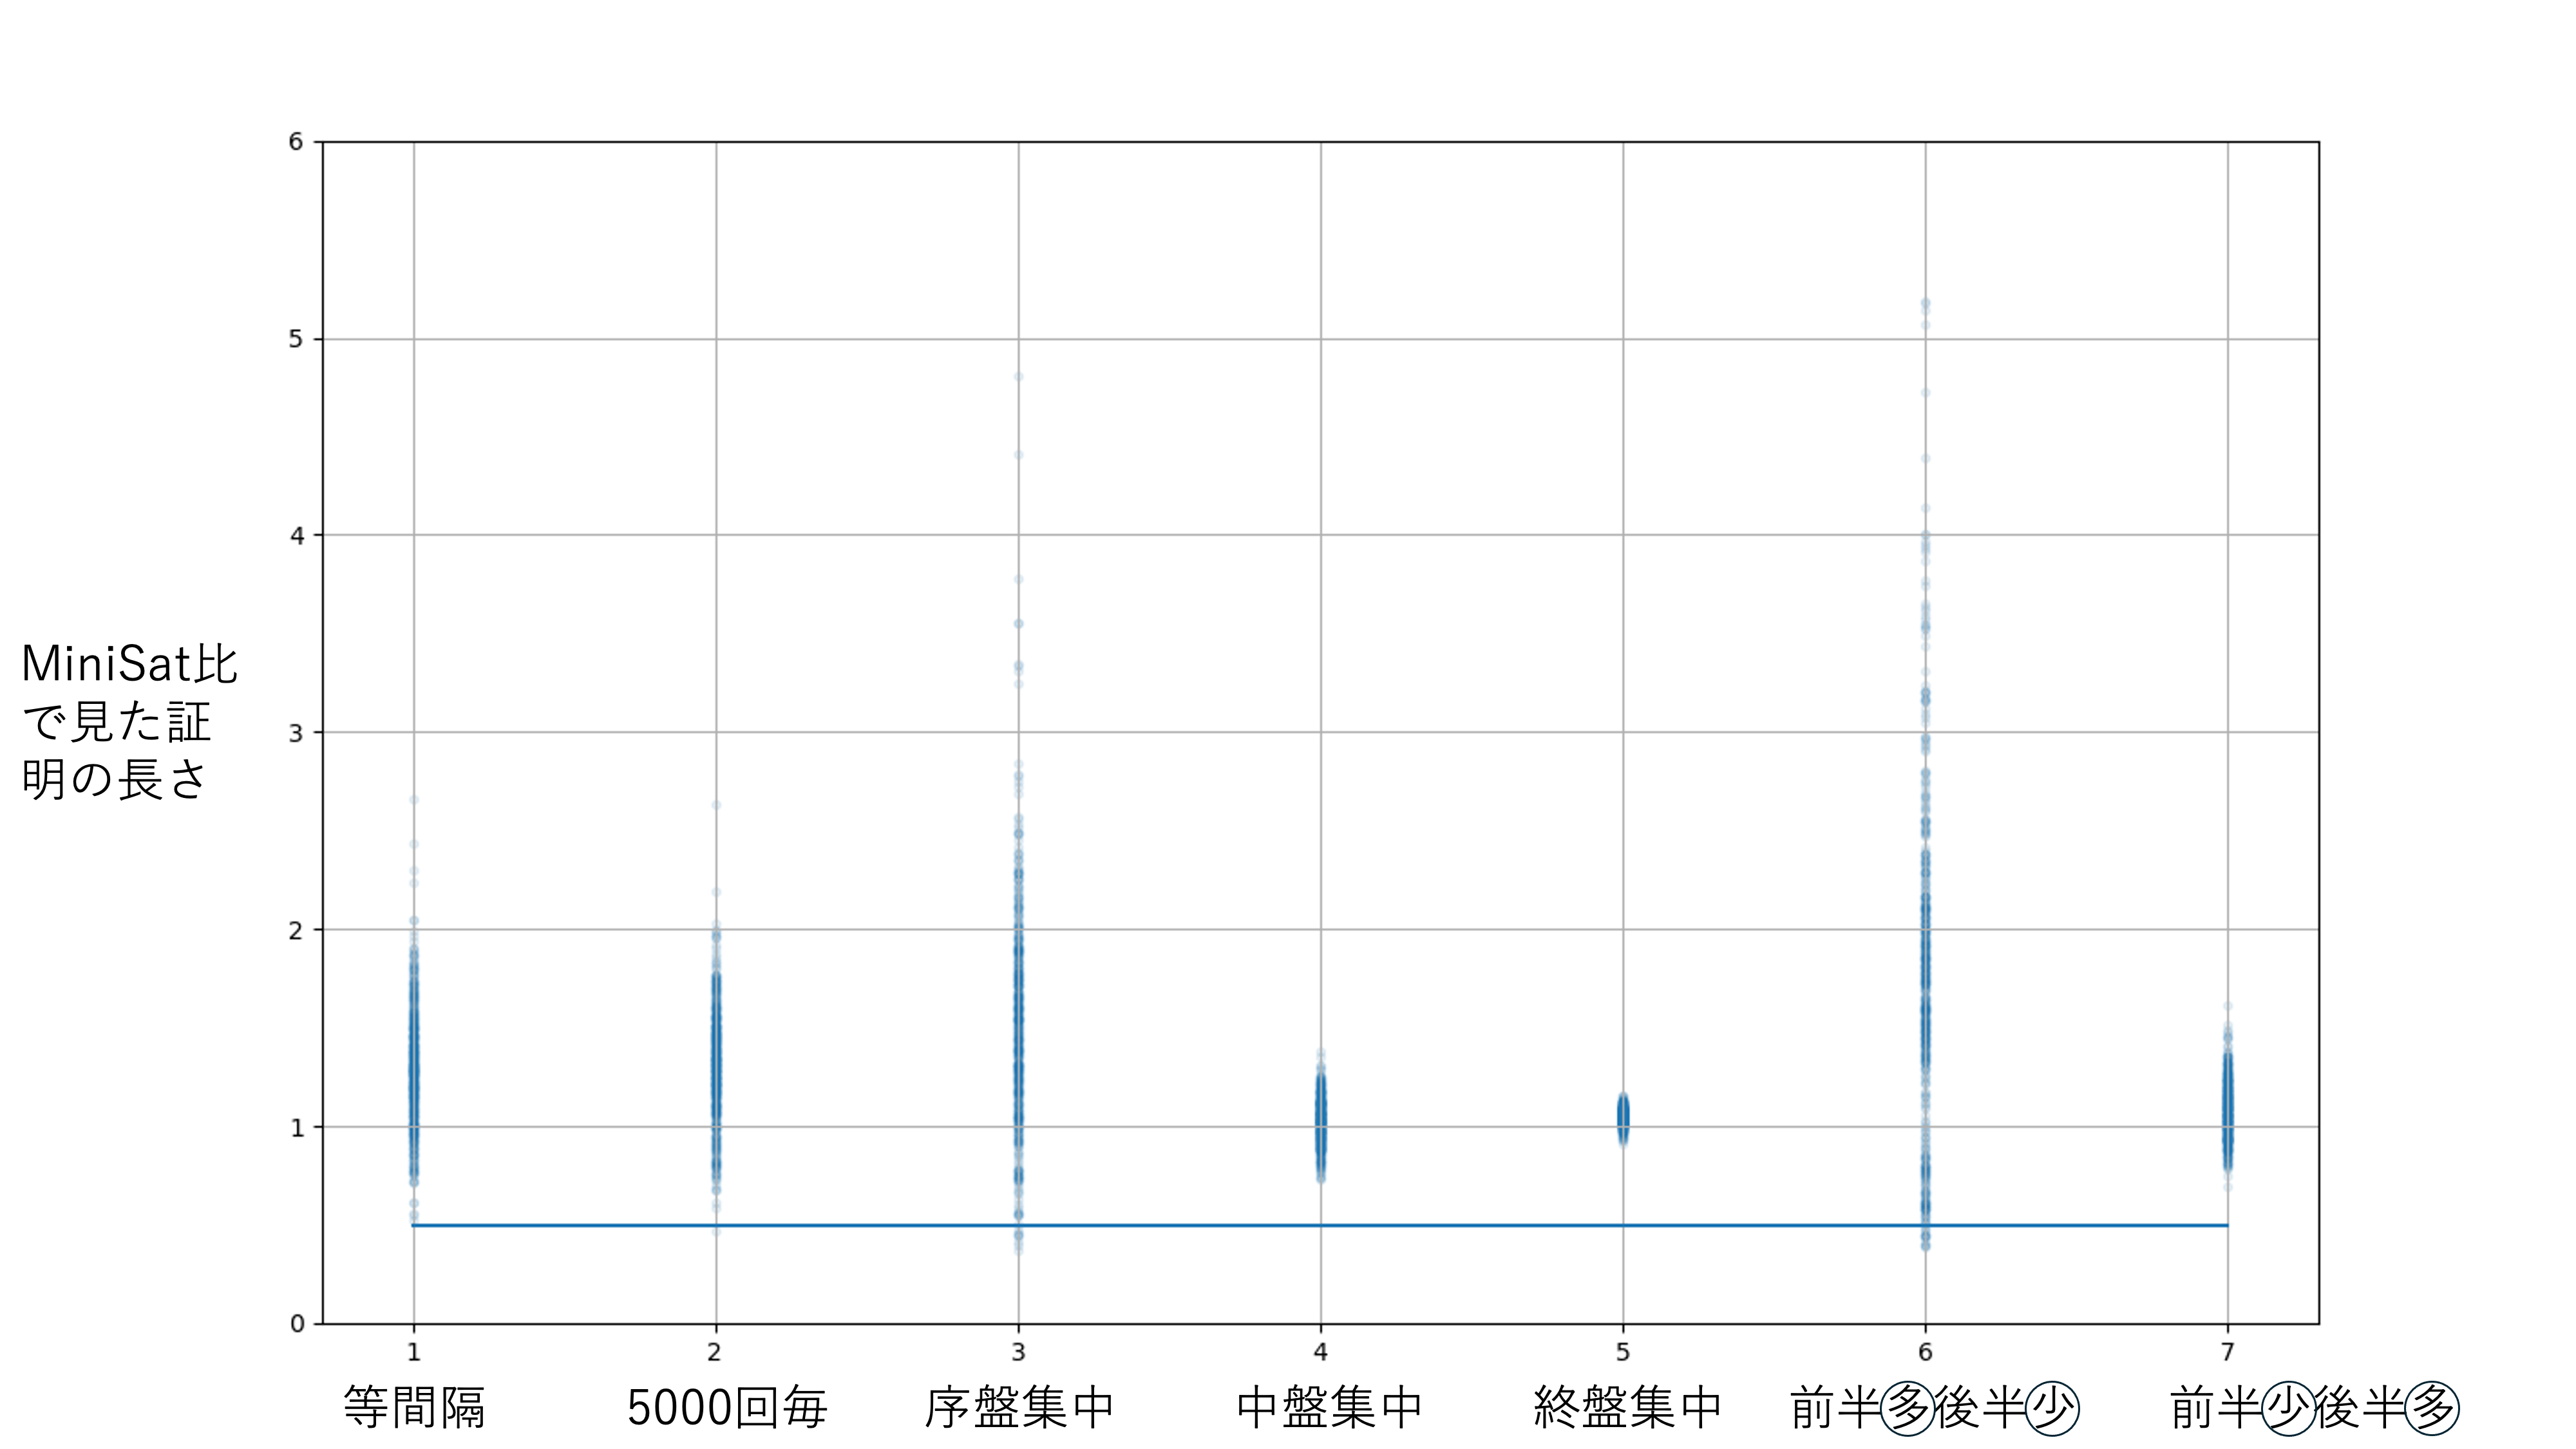
\includegraphics[width=10cm]{figures/Experiment0/1.png}
    \caption{タイミングずらしつつ8回介入(あとでちゃんとした画像に)}
\end{figure}





\subsection{パラメータ調整}%5ページ



まず最初の実験として遺伝アルゴリズムのパラメータ調整を行う実験を行なった。
問題を1つ固定し、遺伝アルゴリズムがより効果的に作用するようにパラメータの調整をしている。
調整を行なったのは以下の4つで、実験によってそれぞれ
\begin{itemize}
    \item 初期集団を作成する際の各染色体の介入数はランダムに選択
    \item 集団のサイズを200
    \item 世代数は30世代
    \item 突然変異を行う際は元の介入の1割を追加・削除
\end{itemize}
といった調整がなされている。
問題はあまり時間がかからない数秒で解けるような問題
\footnote{MiniSatで1.7秒、drat-trimで2.9秒ほどかかる問題で、証明の長さが約25000、変数選択数が約40000回の問題}
を採用した。

% 通常の6000倍ぐらいの実行時間
% 遺伝アルゴリズムはパラメータ調整がが必要


\subsubsection{初期状態}
\begin{figure}[h]
    \centering
    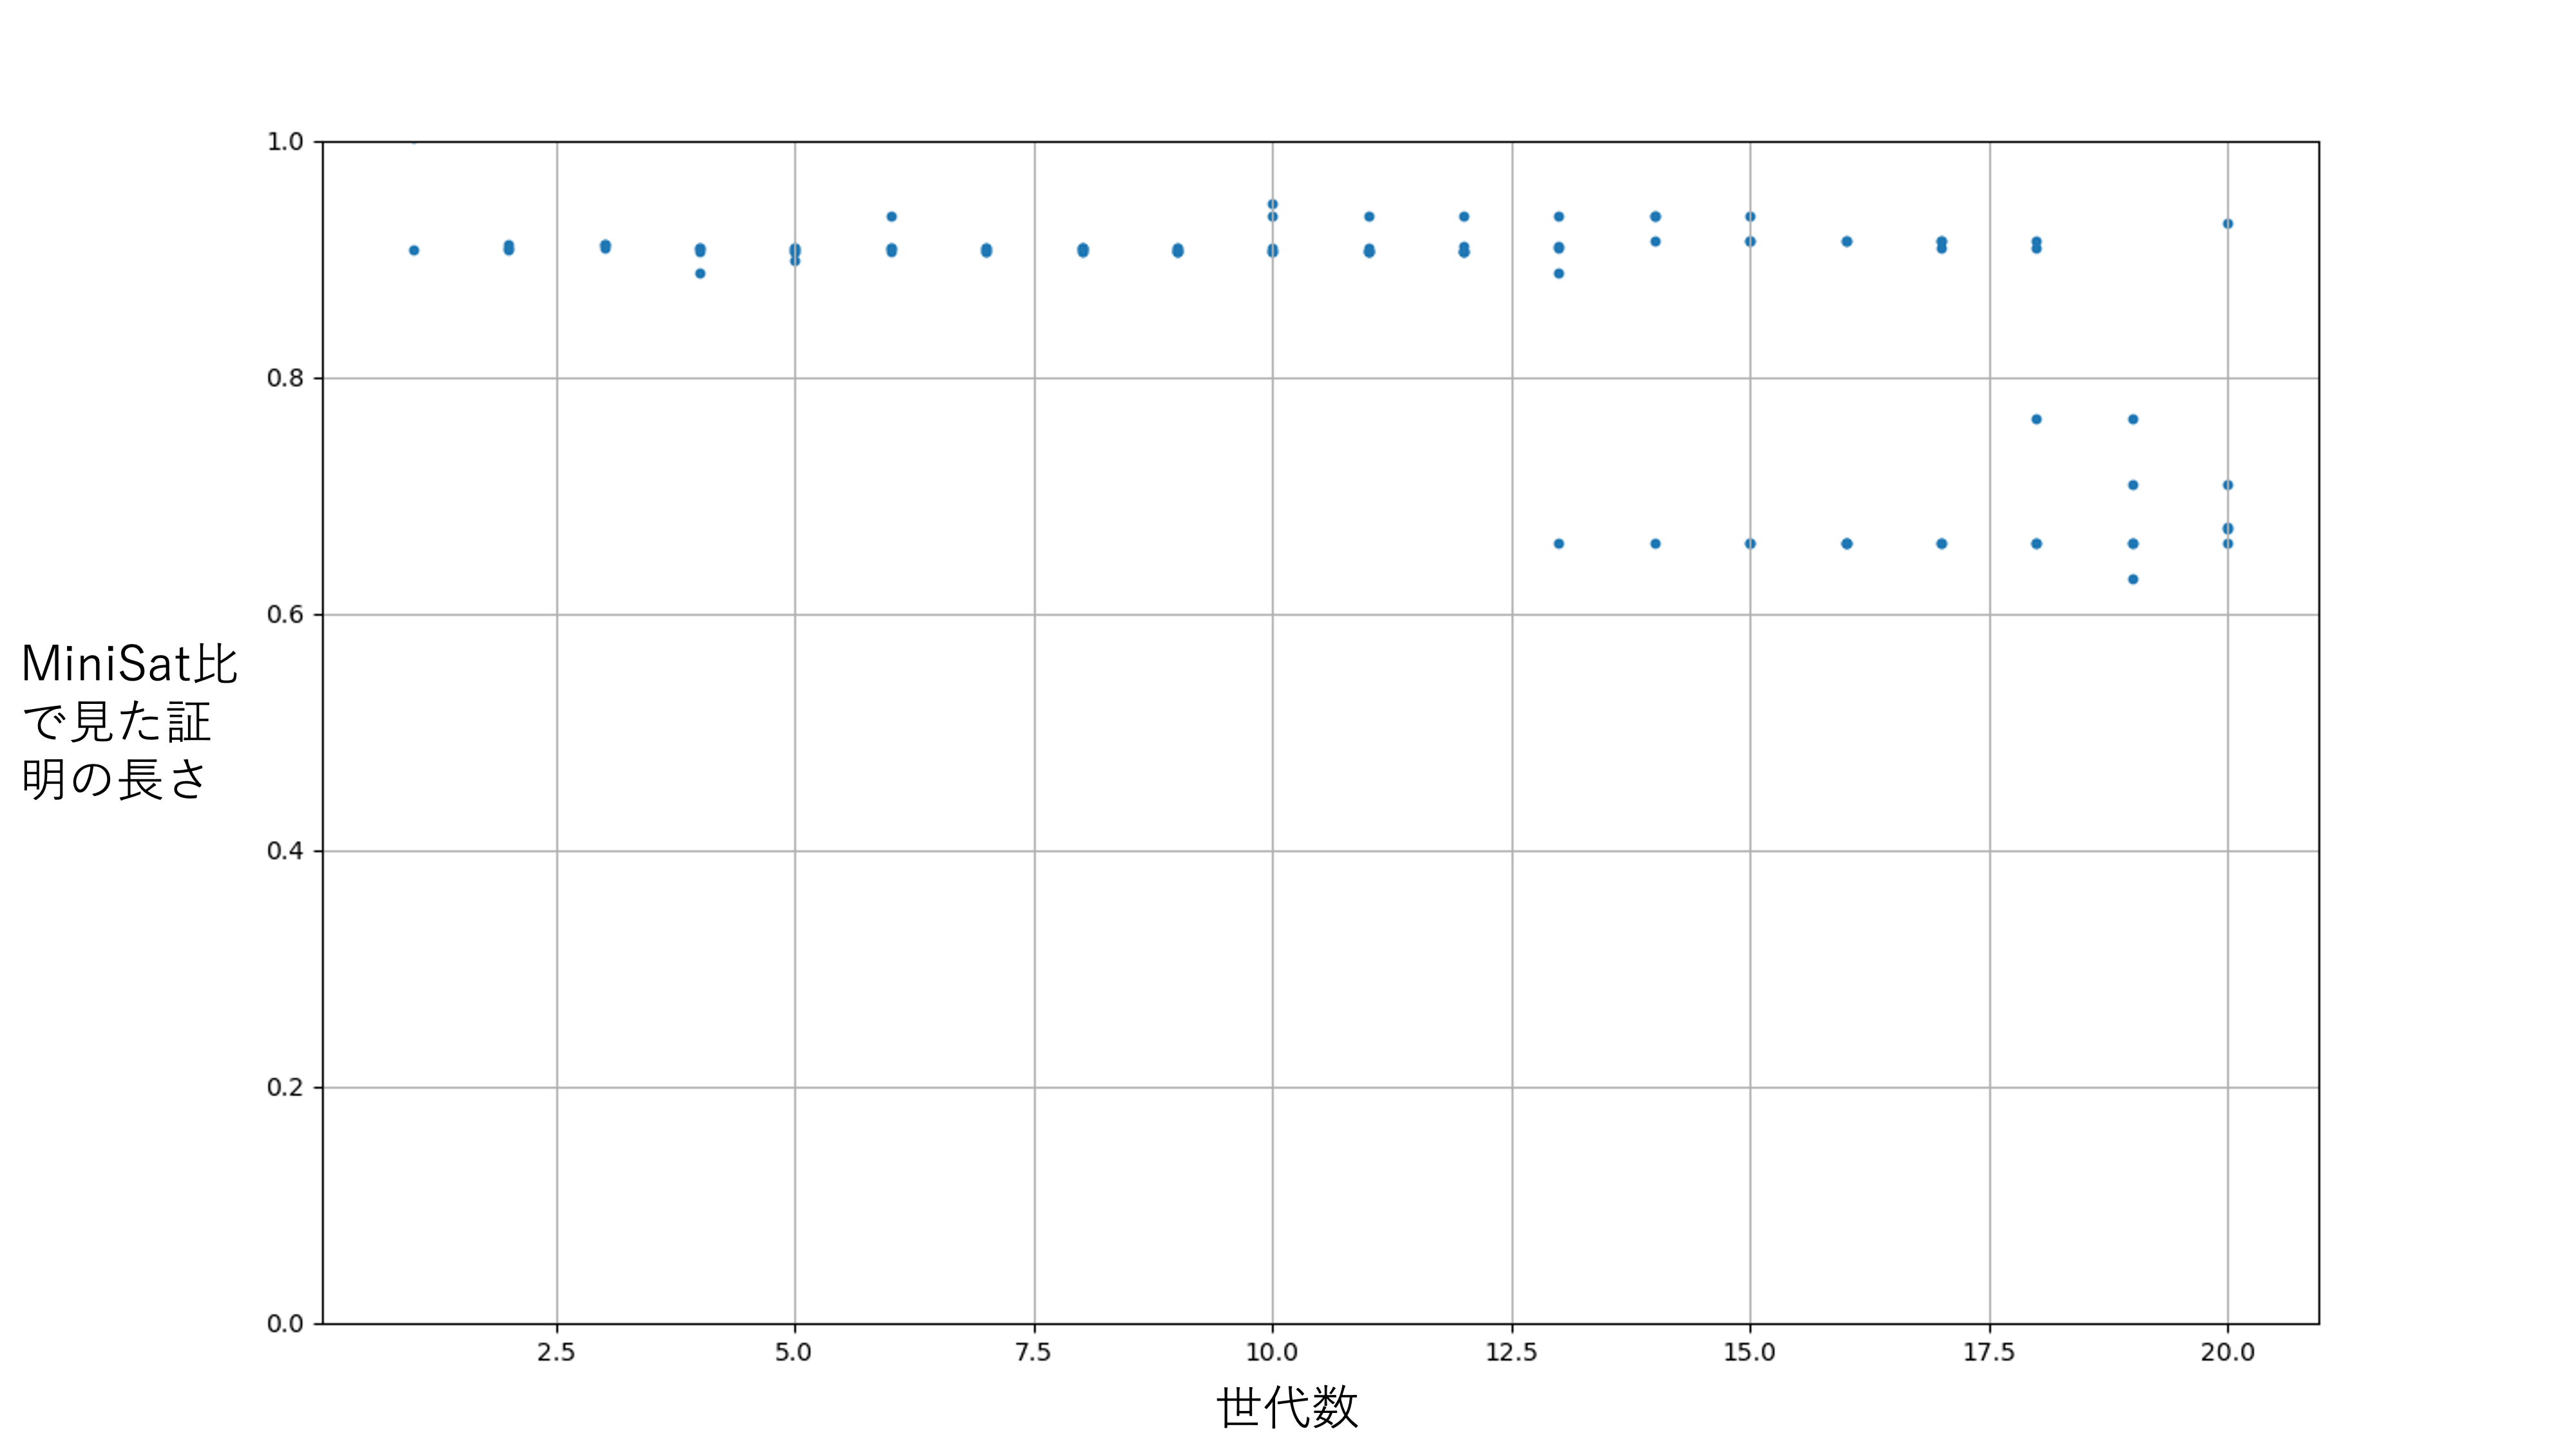
\includegraphics[width=10cm]{figures/Experiment1/1.png}
    \caption{初期パラメータにおける全染色体の証明長}
\end{figure}
最初に現在の遺伝アルゴリズムを実行しその効果を見た。
集団サイズは5で20世代まで作成、初期集団の各染色体の介入の回数は10回で固定し、
突然変異の際の介入の追加・削除数は1としてる。
結果を見ると13世代目で大きく良い個体が作成されているだけで、
それ以外の世代では大きく良い個体が作成されているような箇所はない。
また各染色体に距離があり、集団のサイズが少なく多様性がないように感じられる。
そのため次に集団の多様性を上げるような調整を行なった。
なお、ここでの一番短い証明はもとの証明の60\%ほどの証明であった。



\subsubsection{集団サイズと世代数を増加}
\begin{figure}[h]
    \centering
    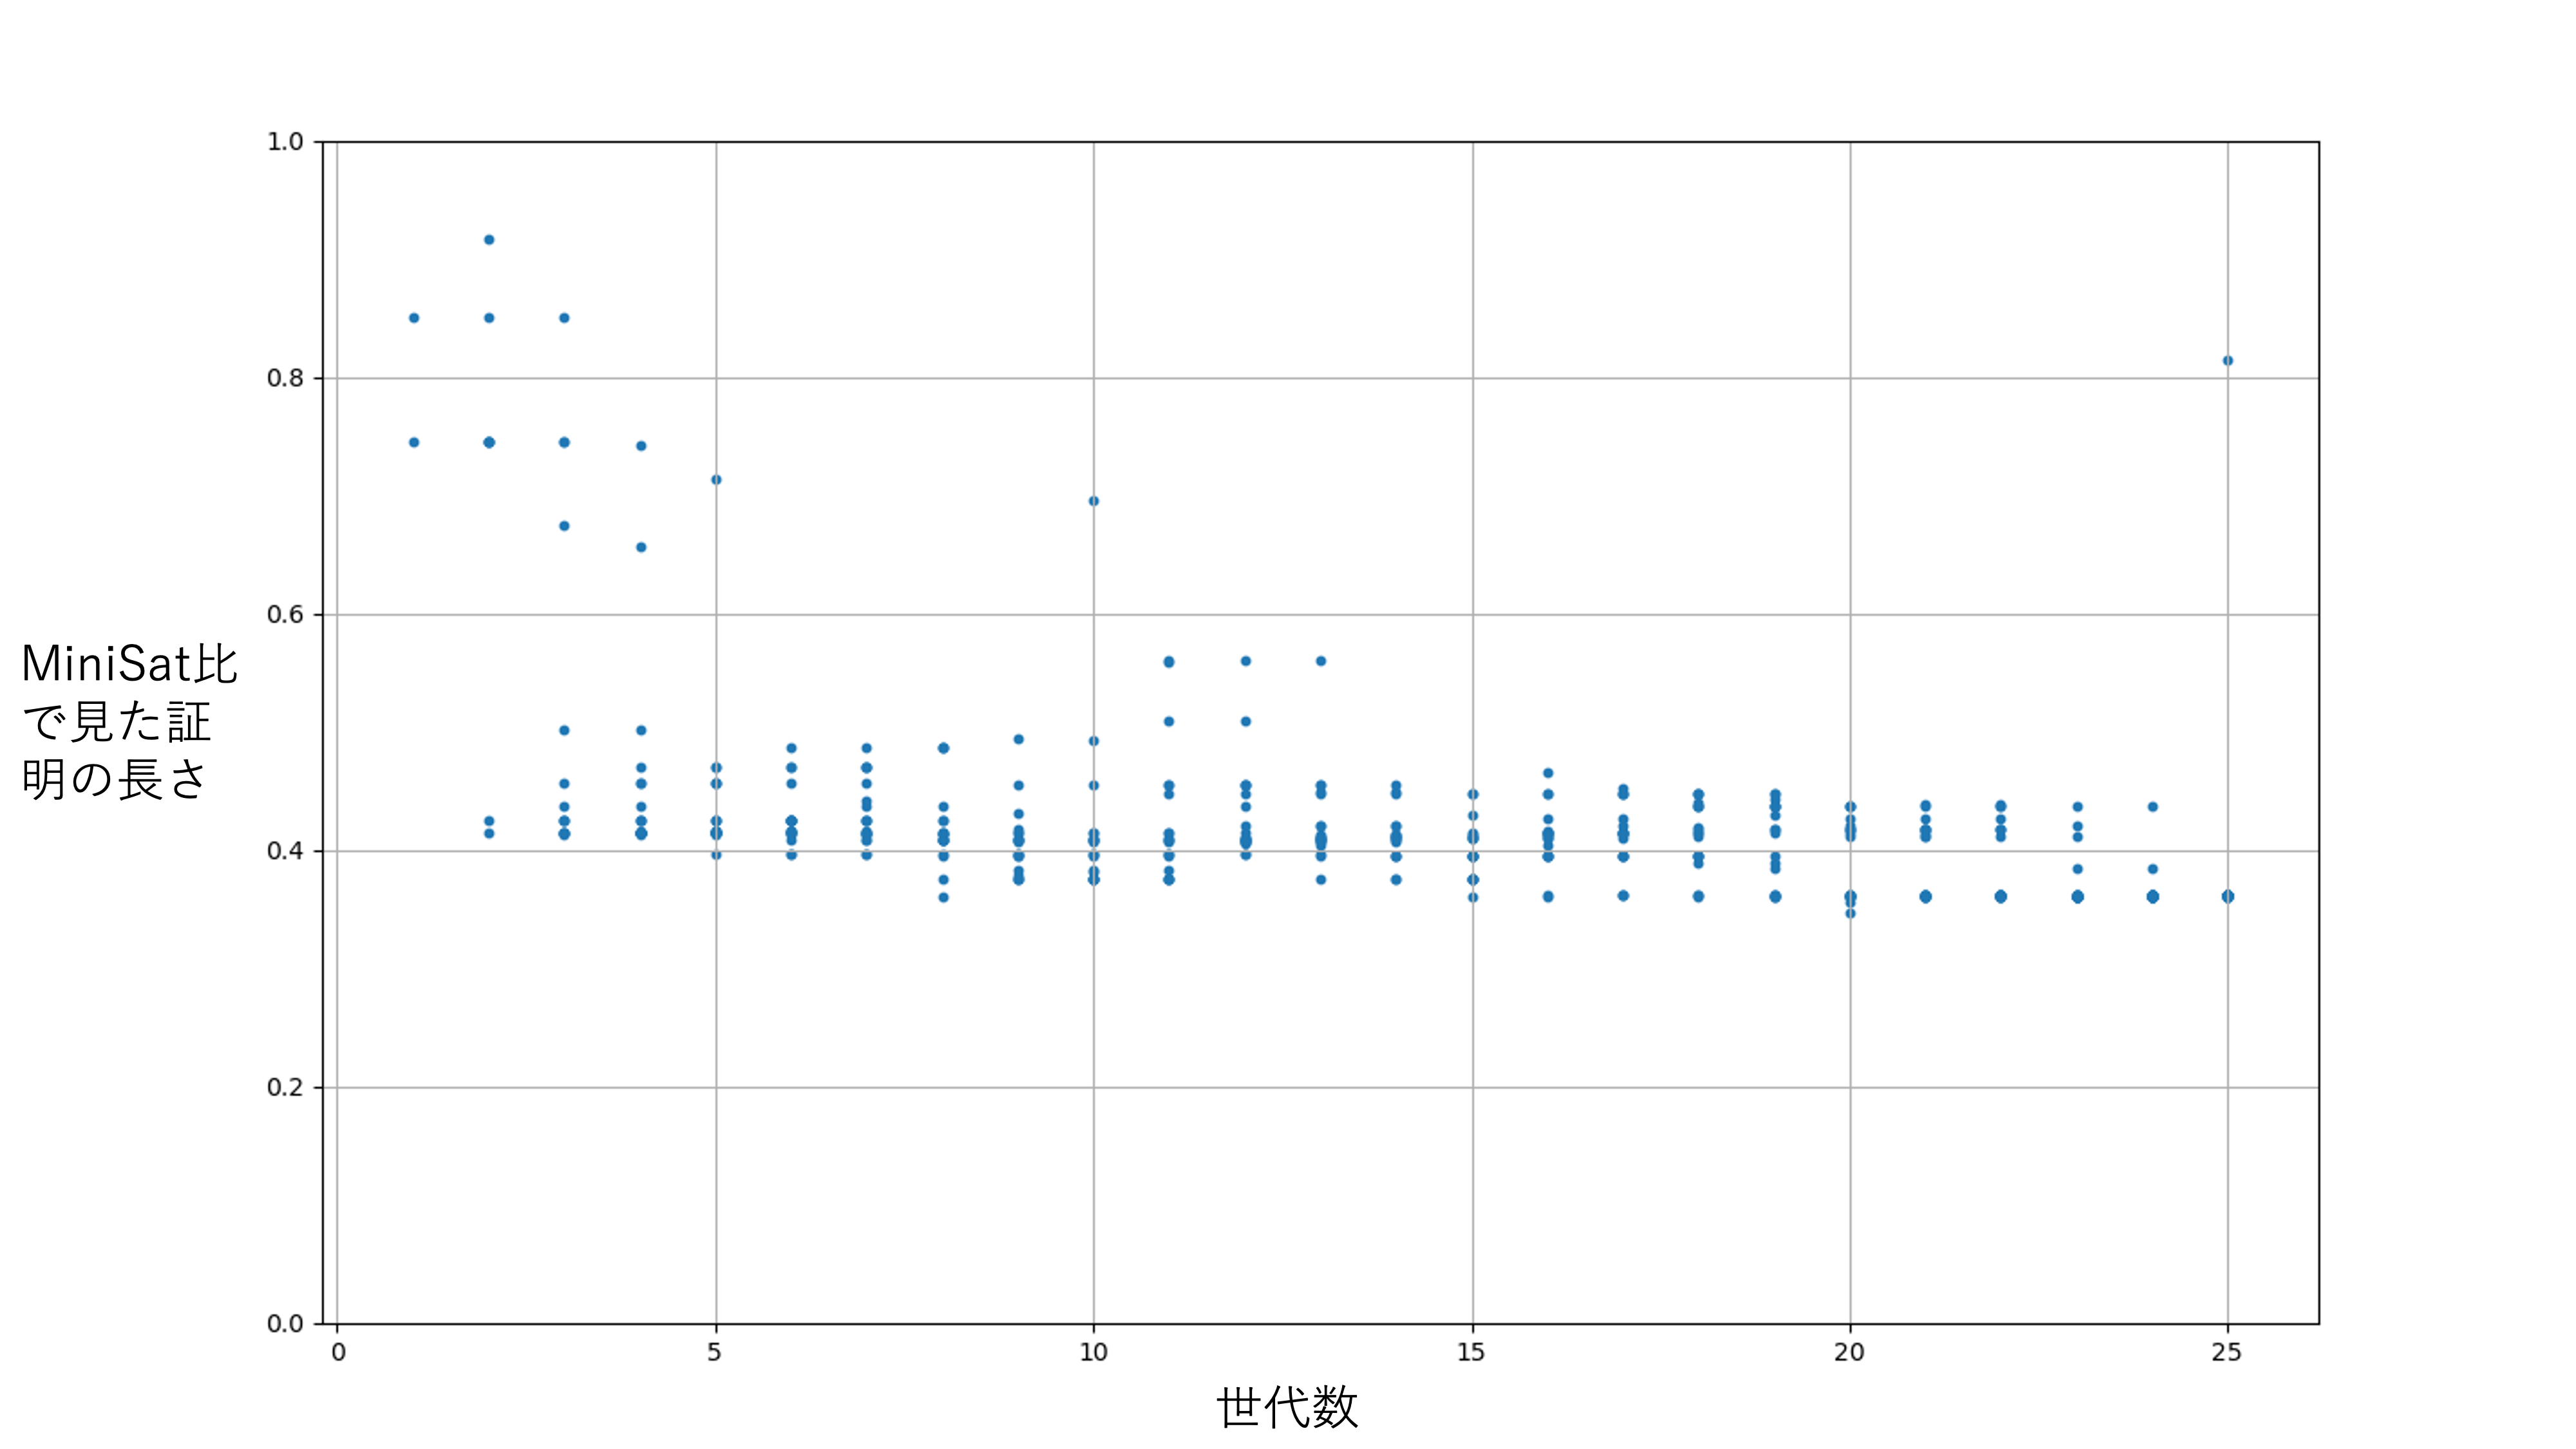
\includegraphics[width=10cm]{figures/Experiment1/2.png}
    \caption{集団サイズと世代を増加}
\end{figure}
次の実験では集団のサイズと世代数を増やす調整を行なった。
ここでは集団のサイズを20、世代数を25にして増やした上で遺伝アルゴリズムを実行した。
この変更によって集団の多様性が増え、より短い証明が作成されることを期待している。
結果として初期の結果よりも短い証明を作成することができた。
2世代目で良い個体を作ることができているが、
5世代目以降ではほとんどの個体が50\%弱のあたりに集まる形になっており、すぐに収束してしまっている。



\subsubsection{介入の回数をランダムに}

 ・20 * 25

 ・初期介入回数ランダム

\begin{figure}[h]
    \centering
    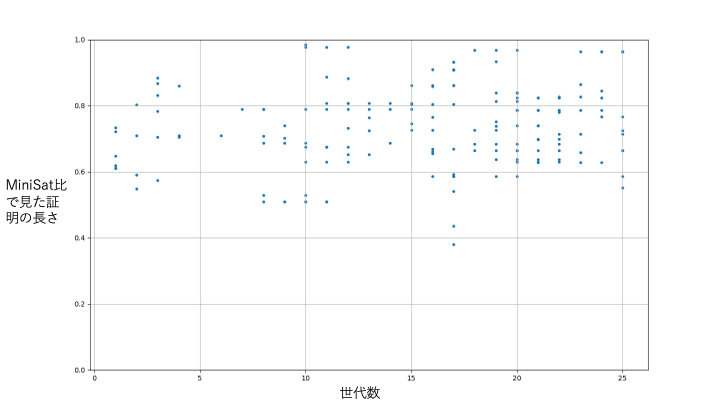
\includegraphics[width=10cm]{figures/Experiment1/3.png}
    \caption{初期の介入回数をランダムに}
\end{figure}

 ・多様性が増えた

 ・どの介入もなんか収束してそう

\begin{figure}[h]
    \centering
    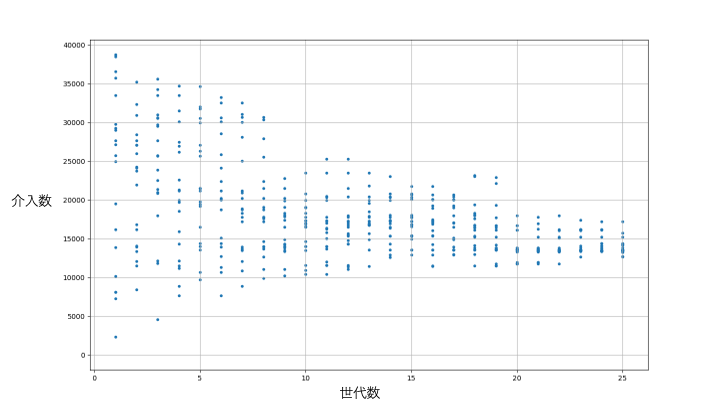
\includegraphics[width=10cm]{figures/Experiment1/3-1.png}
    \caption{介入回数の遷移}
\end{figure}

  ・初期の介入回数を10000以上20000以下に

\begin{figure}[h]
    \centering
    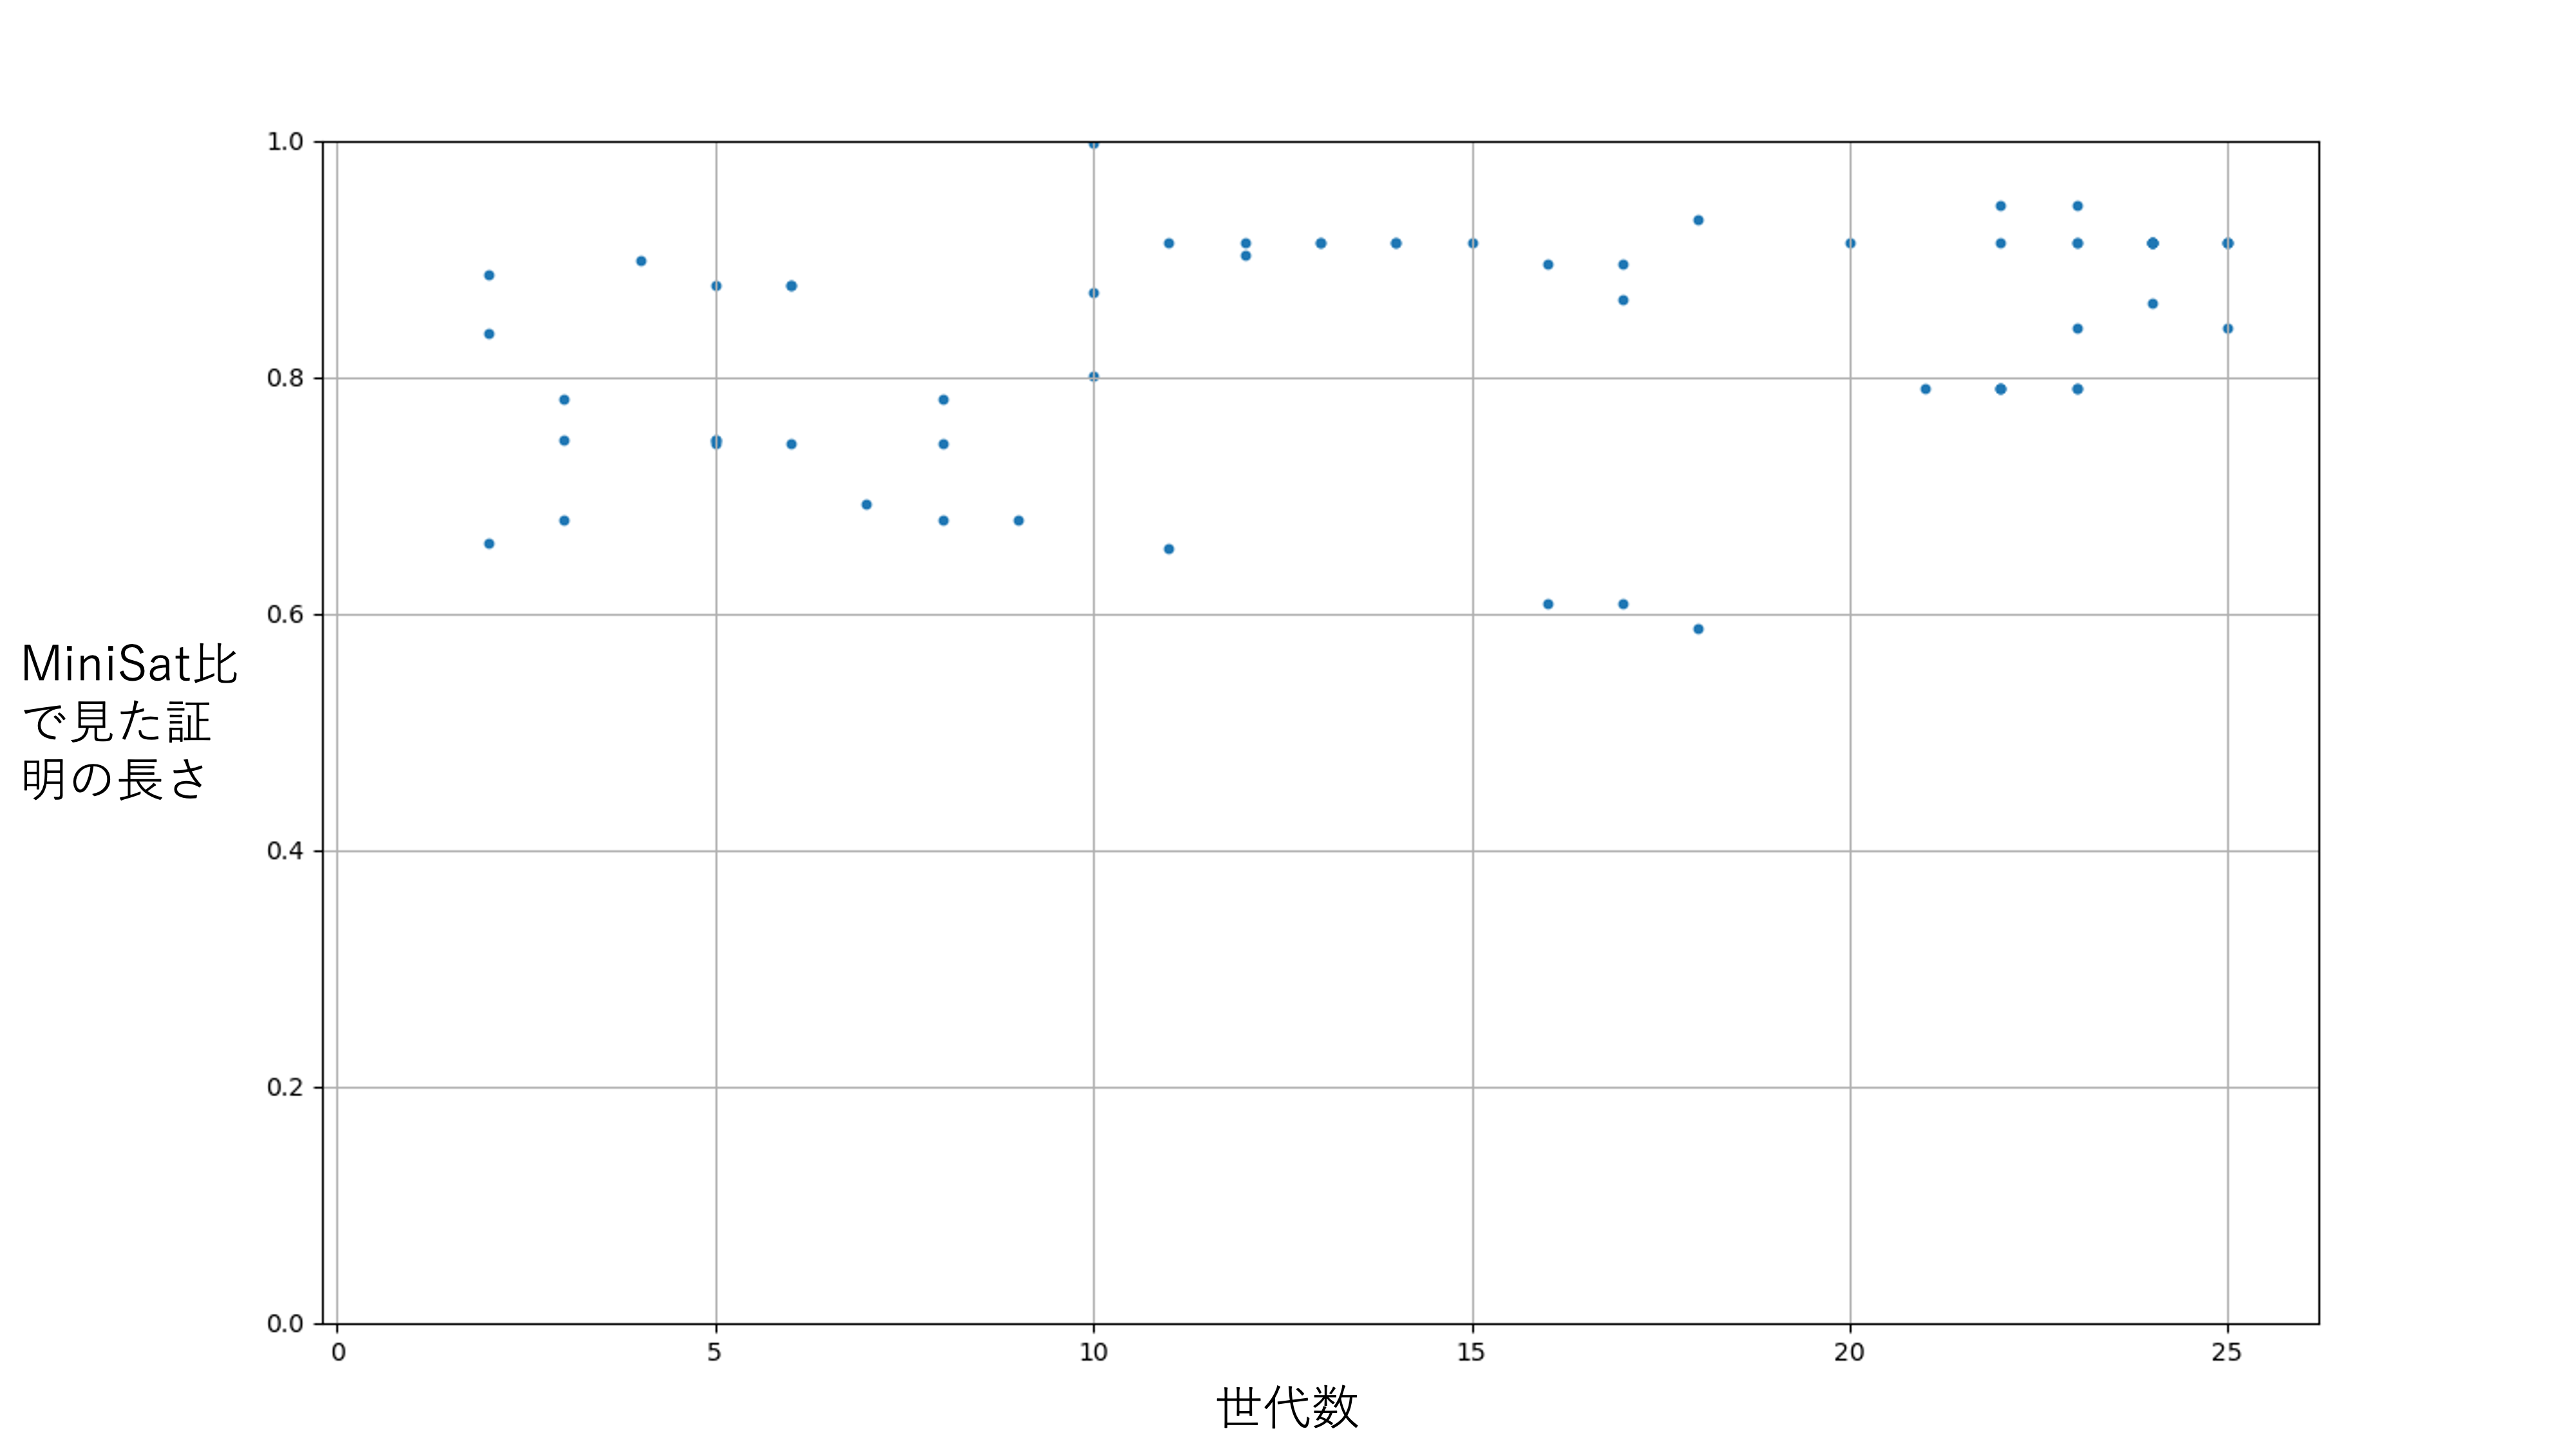
\includegraphics[width=10cm]{figures/Experiment1/3-2.png}
    \caption{介入回数を10000以上20000以下で始める}
\end{figure}

・介入をランダムにしてその状態での集団サイズと試行回数を調べた

4集団サイズと世代の変更

\begin{figure}[h]
    \centering
    \begin{minipage}{0.43\columnwidth}
        \centering
        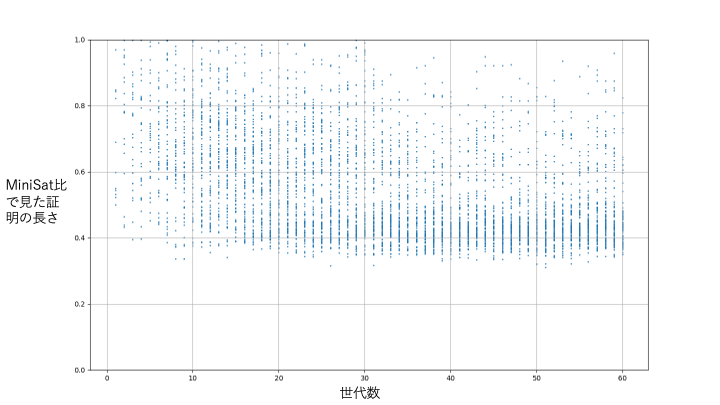
\includegraphics[width=\columnwidth]{figures/Experiment1/4-1.png}
        \caption{集団サイズ100、世代数60}
        \label{fig:サンプルA}
    \end{minipage}
    \hspace{5mm}
    \begin{minipage}{0.43\columnwidth}
        \centering
        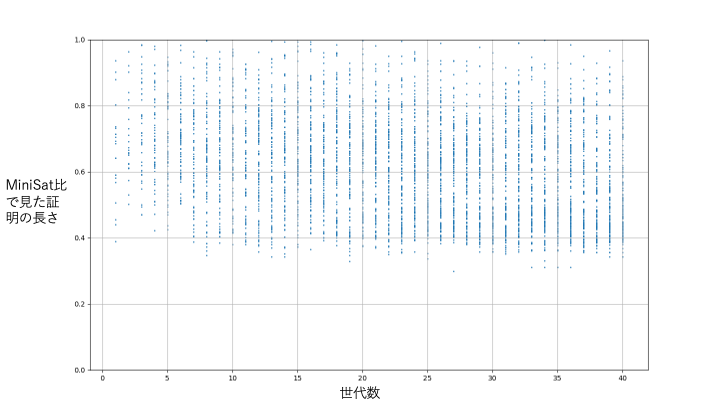
\includegraphics[width=\columnwidth]{figures/Experiment1/4-2.png}
        \caption{集団サイズ150、世代数40}
        \label{fig:サンプルB}
    \end{minipage}
  
    \vspace{3mm}
    
    \begin{minipage}{0.43\columnwidth}
        \centering
        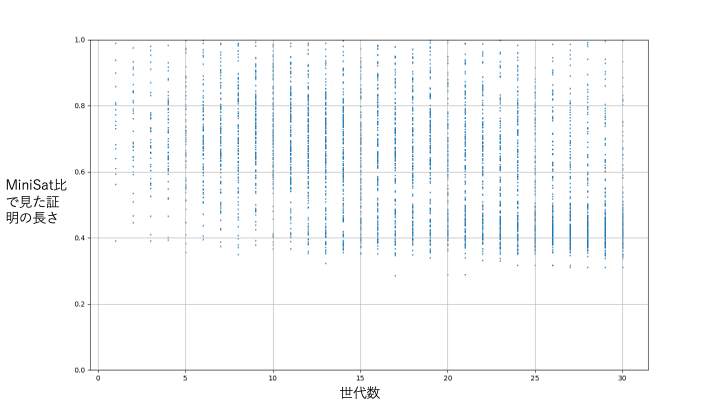
\includegraphics[width=\columnwidth]{figures/Experiment1/4-3.png}
        \caption{集団サイズ200、世代数30}
        \label{fig:サンプルC}
    \end{minipage}
    \hspace{5mm}
    \begin{minipage}{0.43\columnwidth}
        \centering
        
\includegraphics[width=\columnwidth]{figures/white.png}
    \end{minipage}
    \caption*{評価回数を6000として集団サイズと世代を変更}
\end{figure}

% 横にランダムと初期状態のベスト置きたい
5突然変異の変更
\begin{figure}[h]
    \centering
    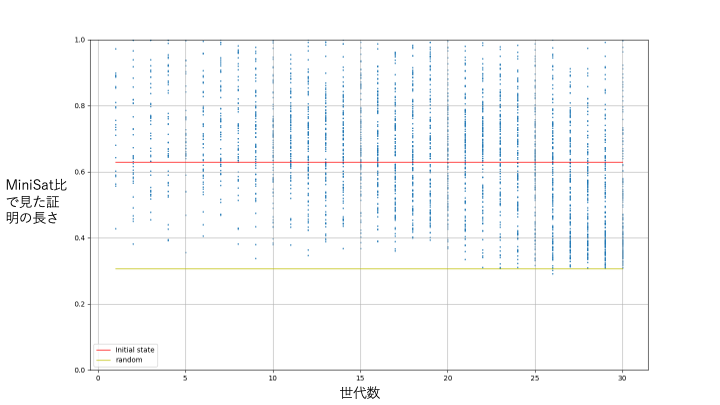
\includegraphics[width=10cm]{figures/Experiment1/5.png}
    \caption{突然変異の変更}
\end{figure}

6ランダムとの比較

7trim前の適応度の比較

 ・実行時間を短縮できないかという目的



\subsection{色々な問題に対して解く}%6ページ

・同じくらいの問題を解く

・長い問題を解く

・各問題のベストを見る

・空いている部分の問題を解く

・学習が続いている問題をを解く



\subsection{kissatとの比較}%4ページ

・kissatとの比較



\subsection{今後のために少し調べたこと}

・適応度を2乗に